\documentclass{article}
\usepackage[utf8]{inputenc}
\usepackage{graphicx}
\usepackage{float}
\usepackage[margin=1.2in]{geometry}

\title{CTA200H 2021 assignment 2}
\author{Rosalind Liang }
\date{May 2021}

\begin{document}

\maketitle

\section{Numerical approximation of a derivative}
\subsection{Methods}
To numerically estimate the derivative at a given point x0, I defined a derivation function taking the the original function (sin(x)), x0 (.1), and stepsize (h), and outputting the value of the taylor expansion with these parameters. Next I created an array of h values spanning from .01 to 1 and passed each value in the array through the derivation function. For each resulting numerical derivative, I used the formula for error to compare against the analytical derivative (cos(.1)). Finally, I used matplotlib to plot the values of h against error (figure 1).

\subsection{Results}
As seen in Figure 1, we observe that as h increases, the numerical estimation of the derivative strays further and further from the analytical solution in an exponential like curve. This makes sense since larger values of h mean straying further and further from the local region around x0.

\begin{figure}[H]
    \centering
    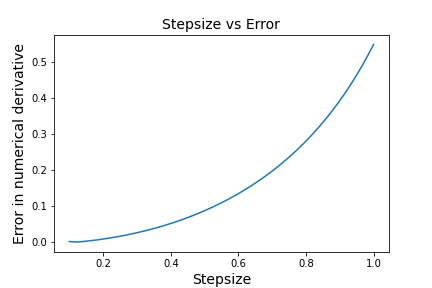
\includegraphics[width=4.5in]{fig1.png}
    \caption{Caption}
\end{figure}


\newpage
\section{Divergence of functions in the complex plane}
\subsection{Methods}

Part 1: To locate the coordinates for which the sequence diverges, I used a for loop to pass through 100 iterations of the sequence and collected points of divergence with np.nan(z), which recognizes when either the real or imaginary component of z is no longer a recognizable number (suggesting divergence to infinity). Matplotlib was then used to plot these coordinates (figure 2). 

Part 2: A similar for loop  was used with np.isfinite(z) to count the number of iterations each coordinate took before diverging. For cases where divergence did not occur within 100 iterations, a special value of -20 was assigned to create contrast in the colourmap, before plotting with matplotlib again (figure 3).

\subsection{Results}
The resulting plot of part 1 is shown in Figure 2, where all points of divergence are in yellow and points that remain bounded are in purple. The plot for part 2 is shown in Figure 3, where all bounded points are in purple and the rest of the plot is a colourmap of each point's divergence iteration. We observe a fractal shaped zone where the sequence stays bounded, ranging from -1 to 1 in the complex axis and -2 to .5 in the real axis. In figure 2, we see that iterations of divergence are significantly higher around the contours of this zone, and drop to approach zero moving away from it. 

\begin{figure}[!htb]
   \begin{minipage}{0.48\textwidth}
     \centering
     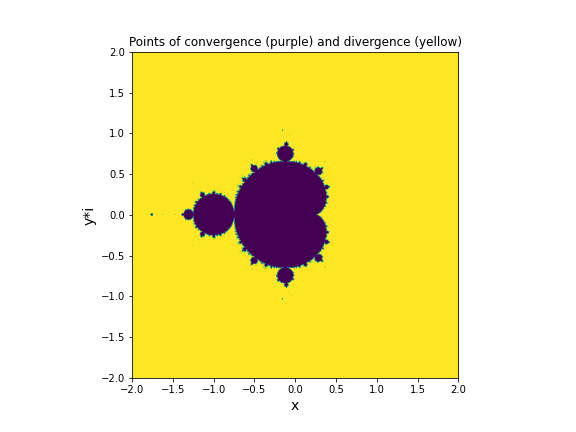
\includegraphics[width=1.1\linewidth]{fig21.png}
     \caption{Convergent vs divergent zones}
   \end{minipage}\hfill
   \begin{minipage}{0.48\textwidth}
     \centering
     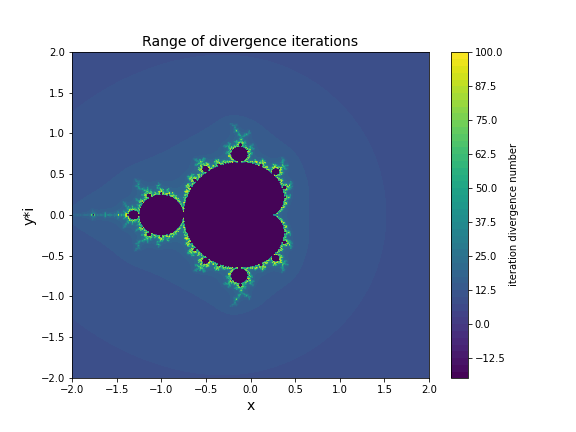
\includegraphics[width=1.1\linewidth]{fig22.png}
     \caption{Divergence iteration number}
   \end{minipage}
\end{figure}


\newpage
\section{The SIR model}
\subsection{Methods}

To integrate each of the ODE's, I defined the model as a function and used odeint from scipy to perform the integration. I then played around with different values of $\beta$ and $\gamma$ before selecting a few which generated interesting plots.

\subsection{Results}
An important observation is that $\beta$ is the rate of infection and $\gamma$ is the rate of recovery. In real life pandemic applications, $\beta$ is almost always greater than $\gamma$. As shown in figures 4-6, the ratio between $\beta$ and $\gamma$ determines the total proportion of the population infected, as well as the time it takes for the recovered population to plateau. Figure 7 shows a case where $\gamma$ is 0, meaning the entire population is quickly infected with no one ever recovering.

\begin{figure}[!htb]
   \begin{minipage}{0.48\textwidth}
     \centering
     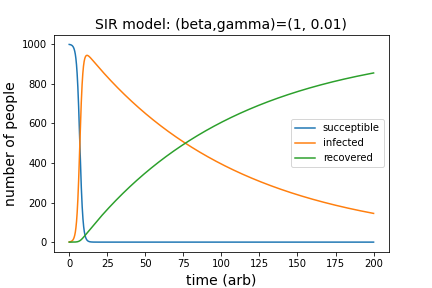
\includegraphics[width=1\linewidth]{fig31.png}
     \caption{infection:recovery = 1:.001}
   \end{minipage}\hfill
   \begin{minipage}{0.48\textwidth}
     \centering
     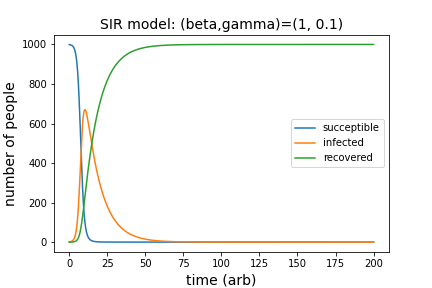
\includegraphics[width=1\linewidth]{fig32.png}
     \caption{infection:recovery = 1:.01}
   \end{minipage}
   \begin{minipage}{0.48\textwidth}
     \centering
     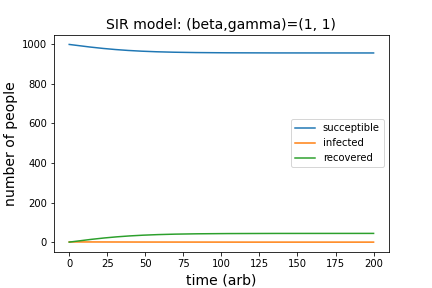
\includegraphics[width=1\linewidth]{fig33.png}
     \caption{infection:recovery = 1:1}
    \end{minipage}
      \begin{minipage}{0.48\textwidth}
     \centering
     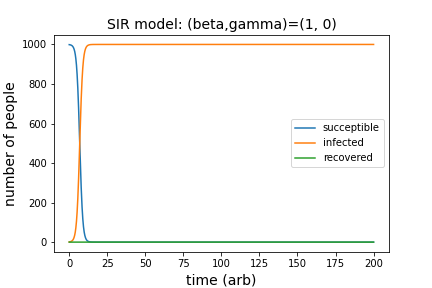
\includegraphics[width=1\linewidth]{fig34.png}
     \caption{infection:recovery = 1:0}
    \end{minipage}
\end{figure}
\end{document}
